Before delving into the mathematical modelling of the quadcopter, it is important to understand a few basic concepts in regards to the working principles of a drone and the frames in which the final model will be defined.

\section{Systems of coordinates} \label{2.1} 
Describing the movement of the quadcopter in a three dimensional space can be done by using two frames, which can be seen in Figure \ref{frames1}. The NED frame is the one that we refer to in our daily life. It points towards North, East and Downwards normal to the surface of Earth. The origin of the NED coordinate system is fixed in O. The frame can also be referred to as inertial and the vectors expressed in it will be marked with $^{I}$. The other frame is fixed on the quadcopter, therefore it is called Body-fixed frame. It has the center in $O_{C}$, which is the center of mass of the drone. Its three axis are x, y and z. The x axis points towards one of the motors, the z axis points to the ground and the y axis completes the orthogonal coordinate system. The vectors described in this frame will be marked with $^{B}$ \cite{Report1} \cite{Report2} .

\begin{figure}[H]
  \centering
    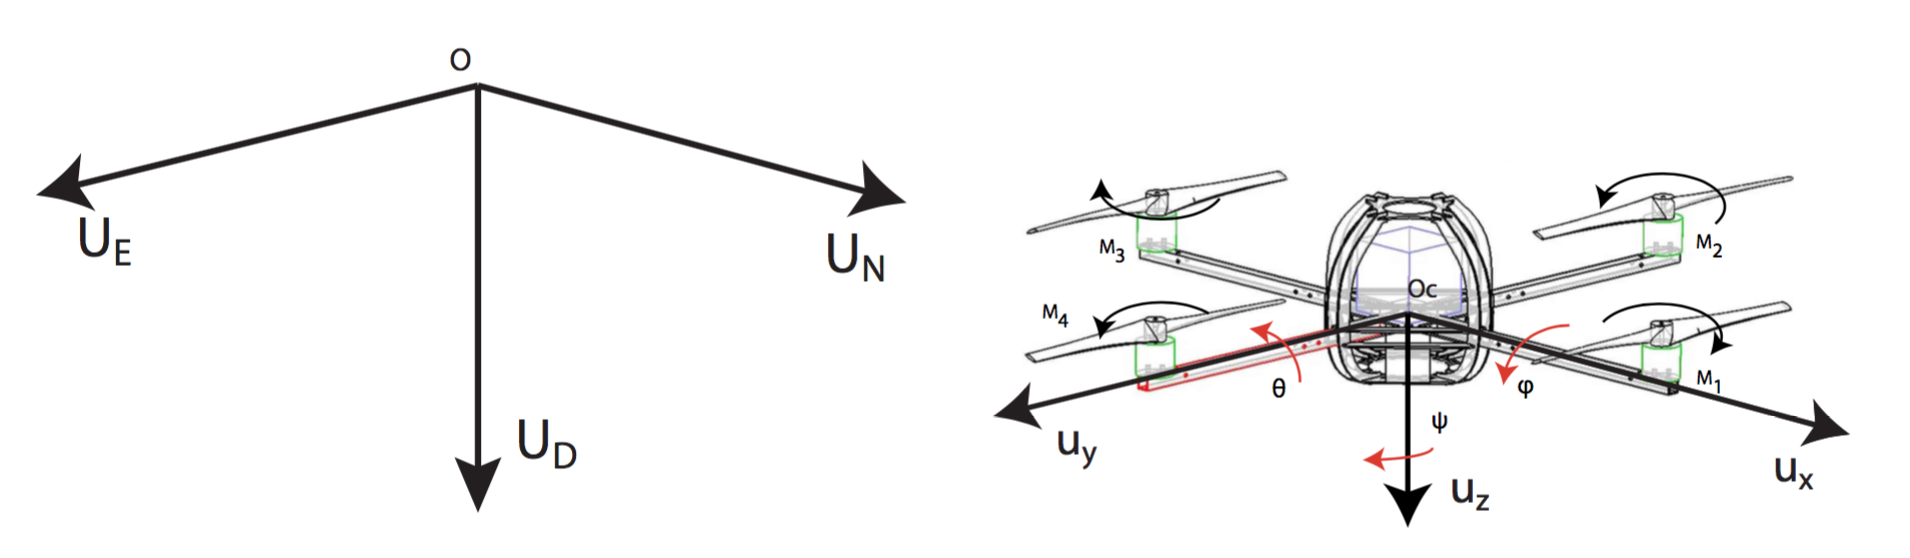
\includegraphics[width=0.9\textwidth]{images/frames1.png}
	\caption{Inertial and Body-fixed Frames.}
	\label{frames1}
\end{figure}

Besides the coordinate system, Figure \ref{frames1} also shows the hexagonal placement of the four motors, the spinning direction of each of them and the roll - $\phi$, pitch - $\theta$ and yaw - $\psi$ angles. 

The quadcopter's position represents the O to $O_{C}$ displacement:

\begin{equation}
	P^{I}=[X, Y, Z] ^{T}
\end{equation} 

The drone's velocity is express as:

\begin{equation}
	V^{B}=[U, V, W] ^{T}
\end{equation} 

The quadcopter's rotation can be described using the 3 Euler angles $\varphi$, $\theta$ and $\psi$ as:

\begin{equation}
	\Psi=[\varphi, \theta, \psi] ^{T}
\end{equation} 

The drone's angular velocity can be expressed using the angular velocity about the $u_{x}$ axis - P, the angular velocity about the $u_{y}$ axis - Q and the angular velocity about the $u_{z}$ axis - R:

\begin{equation}
	\Omega^{B}=[P, Q, R] ^{T}
\end{equation} 

\section{Working principle}

To have an understanding of how an aerial vehicle actually works like, it is important to know the forces affecting it. See Figure \ref{droneForces}.

\begin{figure}[H]
  \centering
    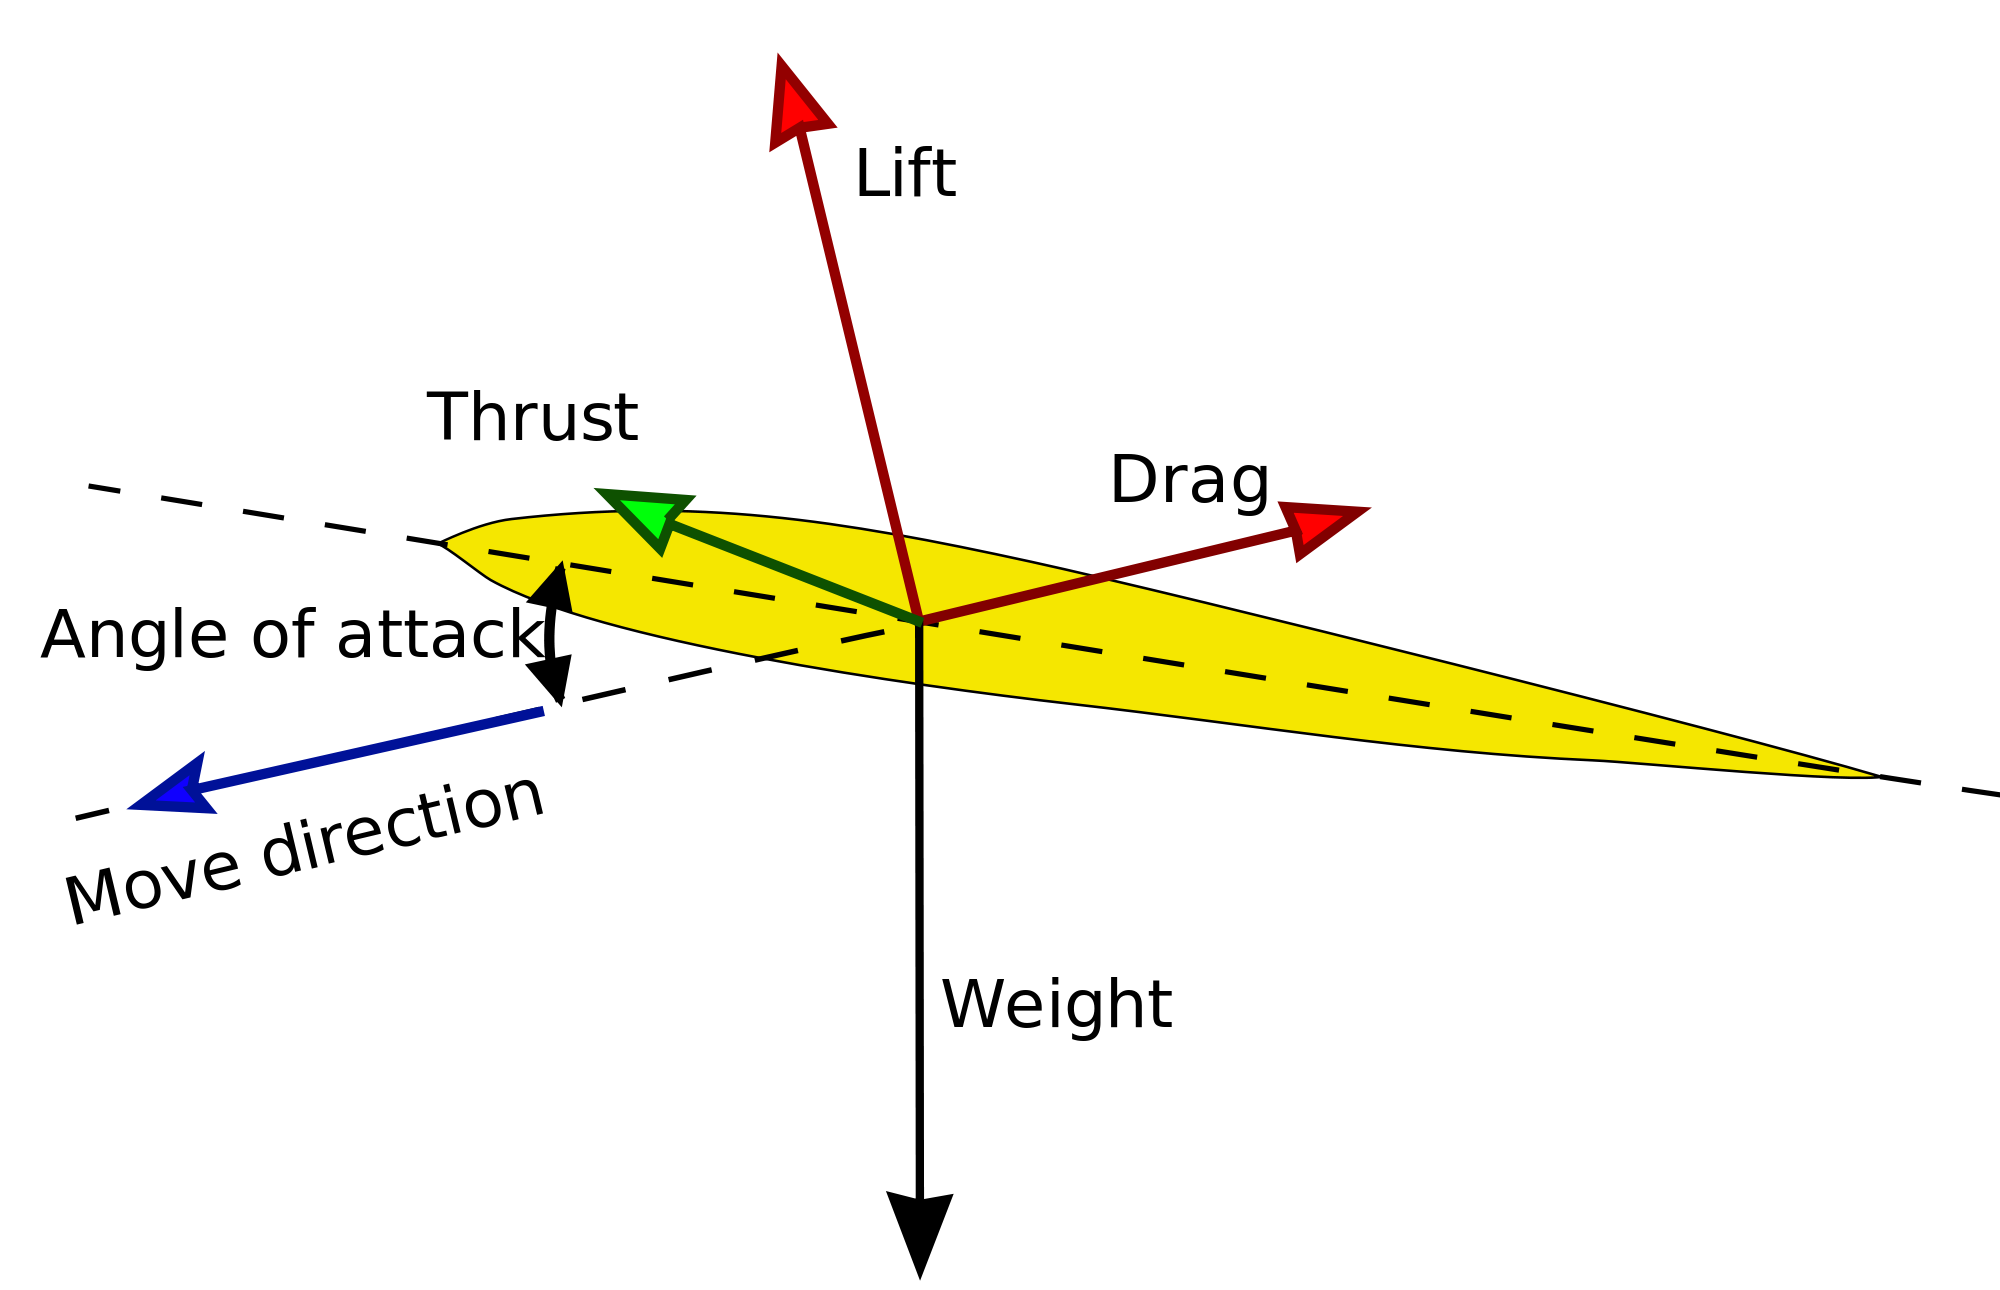
\includegraphics[width=0.75\textwidth]{images/forces.png}
	\caption{Forces Affecting an Aerial Vehicle \cite{ForcesFig}.}
	\label{droneForces}
\end{figure}

The 4 main forces acting on the quadcopter - or any aerial vehicle, for that matter are:

\begin{itemize}
  \item \textbf{Drop} (gravitational force) affects the vehicle at all times. As any object on Earth, its mass is driven towards the centre of the planet. This force is always expressed as: $F_g = mg$, where \textit{m} is the mass of the drone and \textit{g} is the gravitational constant.
  \item \textbf{Thrust} is the force generated by the motors that is allowing the vehicle to move towards its heading. In the case of a quadcopter, this force only exists when the force generated by the motors is uneven.
  \item \textbf{Lift} is the force created through a difference in the air pressure above and below the motor (according to Bernoulli's principle). Quadcopter's motors constantly generate lift force, which must be higher than the drop force in order for the vehicle to take off.
  \item \textbf{Draw} is the resistance created by the air as the vehicle moves through it. It opposes the thrust force and therefore must be lower than the thrust force in order for the quadcopter to move on. In cases when there is no wind, such as indoors area, this force can be disregarded.
\end{itemize} 

If the motors are powered off, the only force affecting the drone is the drop and therefore the quadcopter stays on the ground. In order to lift it up, we need to understand the relationship between quadcopter and thrust to weight ratio - or TWR for short. This ratio can be determined by equation $F_t/F_g$ and describes the vehicle's ability to move up. With TWR expressed as a number, assuming that each motor generates equal amount of thrust, three cases can be identified:

\begin{itemize}
\item \textbf{TWR<1}: The gravitational force is higher than the lift force and therefore the quadcopter is drawn towards the ground.
\item \textbf{TWR=1}: The forces are equal, causing quadcopter's altitude to stay constant.
\item \textbf{TWR>1}: The thrust is higher than drop force, allowing vehicle to move upwards.
\end{itemize}

Therefore, in order to get a quadcopter up in the air, it is necessary to generate enough thrust for TWR ration to be higher than one. In order to land it, the TWR must be smaller than 1, allowing the quadcopter to move downwards.

\section{Quadcopter maneuvering}
Quadcopters are made with four identical motors, each of them having an attached propeller. As it can be seen in Figure \ref{rollpitchyaw}, each pair of propellers rotate in different directions. The odd numbered motors have clockwise rotation, while even numbered motors have counter-clockwise rotation. The speed of the motors has to be adjusted in order to obtain the maneuvers shown in Figure \ref{rollpitchyaw}. 

\begin{figure}[H]
  \centering
    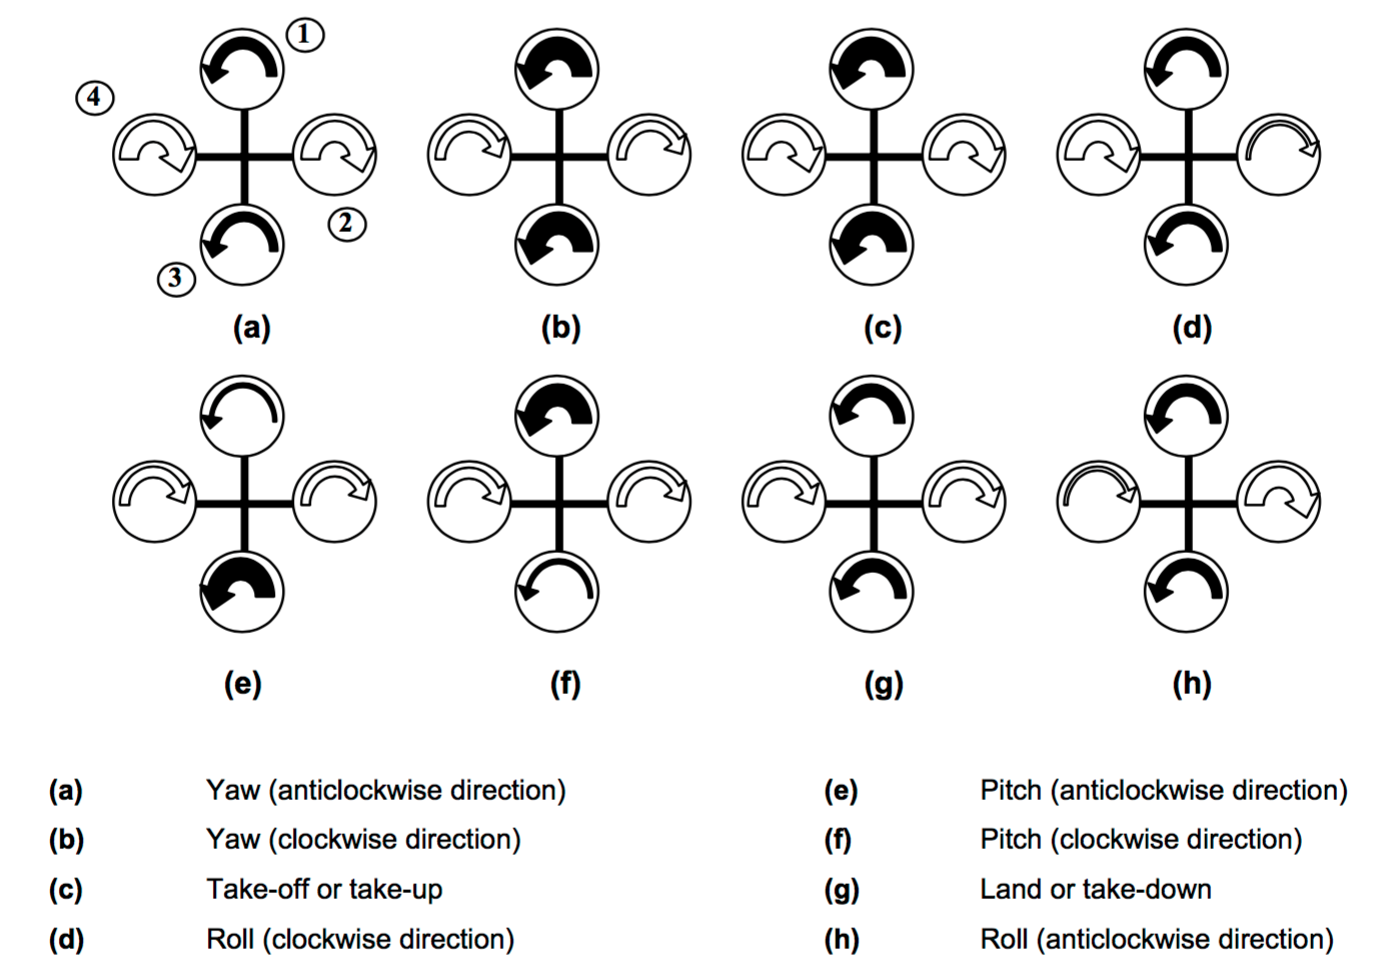
\includegraphics[width=0.9\textwidth]{images/rollpitchyaw.png}
	\caption{Quadcopter Rotation System \cite{RPYFig}.}
	\label{rollpitchyaw}
\end{figure}

The arrows in Figure \ref{rollpitchyaw} represent the angular speeds of the motors and they can be written as:

\begin{equation}
	\omega=[\omega_{1}, \omega_{2}, \omega_{3}, \omega_{4}] ^{T}
\end{equation} 

The quadcopter's possible motions can be split into four categories:

\begin{itemize}
  \item \textbf{Rolling motion} is represented by the rotation of the vehicle about the $u_{x}$ axis and it can be obtained when $\omega_{2}$ and $\omega_{4}$ are manipulated. In order to obtain a positive rolling, $\omega_{4}$ is decreased while $\omega_{2}$ is increased. The opposite will result in a negative rolling motion. Both movements can be seen in cases (a) and (b).
  \item \textbf{Pitch motion} is represented by the rotation of the quadcopter about the $u_{y}$ axis and it can be obtained when $\omega_{1}$ and $\omega_{3}$ are manipulated. In order to obtain a positive pitch, $\omega_{3}$ is decreased while $\omega_{1}$ is increased. The opposite will result in a negative pitch motion. Both movements can be seen in cases (c) and (d).
  \item \textbf{Yaw motion} is represented by the rotation of the drone about the $u_{z}$ axis and it can be obtained by having a difference in the torque developed by each pair of propellers. The torque can be changed by having a bigger angular speed on one of the propeller pairs over the other. Both negative and positive yaw motions can be seen in cases (e) and (f).
  \item \textbf{Translational motion} or vertical movement can be obtained by equally increasind or decreasing the angular speeds of all motors as seen in cases (g) and (h)\cite{Report1}.
\end{itemize} 

\section{Assumptions}
Given the fact that stabilizing a quadcopter is quite a complex problem, we will make a few general assumptions that will enable us to make a more simple version of the model:
\begin{itemize}
  \item The quadcopter is symmetric along $u_{x}$ and $u_{y}$.
  \item The quadcopter is a rigid body.
  \item The flapping effects of the rotors are ignored.
  \item Nonlinearities of the battery are ignored.
  \item Both accelerometer and gyroscope sensors are considered to be at the center of mass of the quadcopter.
  \item All motors have the same time constant.
  \item All aerodynamic forces acting on the quadcopter are ignored.
\end{itemize} 